% !TeX program = lualatex
% !TeX encoding = utf8
% !TeX spellcheck = uk_UA


\documentclass[]{ProblemBook}



\begin{document}

%=========================================================
\begin{problem}%
Струм $I$  тече у додатному напрямку осі $OZ$ декартових координат.
Знайти інтеграл $\int\limits_L \Bfield(\vect{r})\cdot d\vect{r}$ по траєкторії $L$, що показано червоним кольором на рисунку;  $\Bfield$ --- індукція
магнітного поля, створюваного струмом.
\end{problem}

\begin{center}
\begin{tikzpicture}[>=latex,
		midarrow/.style={
				postaction={ decorate,
						decoration={ markings, mark=at position .55 with {\arrow{>}}}}
			},
		sig/.style={font=\scriptsize, text=black},
	]
	\draw[->] (0,0) -- ++(2, 0) node[below] {$y$};
	\draw[->] (0,0) -- ++(225:1.75) node[below] {$x$};
	\draw[->] (0,0) -- ++(0, 2) node[left] {$z$};

	\draw[dashed] (0,0) -- ++(-2, 0);
	\draw[dashed] (0,0) -- ++(225:-1.75);
	\draw[dashed] (0,0) -- ++(0, -2);

	\draw[postaction={ decorate,
				decoration={ markings, mark=at position .7 with {\arrow{>}}}}, ultra thick, gray] (0, -1.75) -- node[pos=0.7, left] {$I$} (0, 1.75);
	\draw[red, thick, midarrow] (-1.5, 0) coordinate (-b) node[sig, above]  {$-b$} -- (-0.5, 0) coordinate (-a) node[sig, above]  {$-a$} -- ++(225:0.5)
	-- ++(1, 0) --
	++(225:-0.5) coordinate (a)
	node[sig, above]  {$a$}  -- ++(1, 0) coordinate (b) node[sig, above]  {$b$};

    \draw (-b) -- +(0,0.1) -- +(0, -0.1)
          (-a) -- +(0,0.1) -- +(0, -0.1)
          (a) -- +(0,0.1) -- +(0, -0.1)
          (b) -- +(0,0.1) -- +(0, -0.1);


    \draw[|-|] (0.65, 0) -- node[pos=0.5, sig, anchor=north west] {$h$} ++(225:0.5);
\end{tikzpicture}
\end{center}
%=========================================================


%=========================================================
\begin{problem}\label{prb:charge_in_hole}
Всередині незарядженої металевої кулі якимось чином зробили сферичну порожнину (див. рис.~\ref{charge_in_hole}), в центрі якої помістили заряд  $q$.
Знайти напруженість електричного поля в усьому просторі.
\end{problem}

	\begin{figure}[h!]\centering
		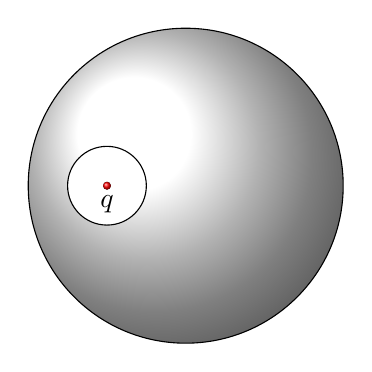
\begin{tikzpicture}
			\draw [ball color=white] (0,0) circle (2);
%			\draw [-stealth] (0,0) -- node[above left] {$R$} (60:2);
			\draw [fill=white] (-1,0) circle (0.5);
			\fill [ball color=red] (-1,0) circle (0.05) node[below] {$q$};
		\end{tikzpicture}
		\caption{До задачі~\ref{prb:charge_in_hole}}
		\label{charge_in_hole}
	\end{figure}

%=========================================================


%=========================================================
\begin{problem}\label{prb:potter}
Заряд $q$ розташований на верхній основі горщика (там, де мала бути кришка) на деякій відстані від осі (рис.~\ref{pic:potter}). Знайти потік вектора
напруженості електричного поля, створюваного зарядом, через бічні стінки та дно горщика. Відстань заряду до осі, параметри, що визначають форму та
розміри горщика задайте самостійно.
\end{problem}


%=========================================================
\begin{problem}\label{prb:tube}
Водопровідна труба має довжину $10$~м та діаметр $5$~см. Заряд $q$ розташований на вході в трубу з лівого кінця (рис.~\ref{pic:tube}).
Знайти потік вектора напруженості електричного поля, створюваного зарядом, через стінки труби з точністю до другого знаку після коми.
\end{problem}

%=========================================================
\begin{figure}[h!]\centering
%---------------------------------------------------------
\begin{minipage}[t]{0.45\linewidth}\centering
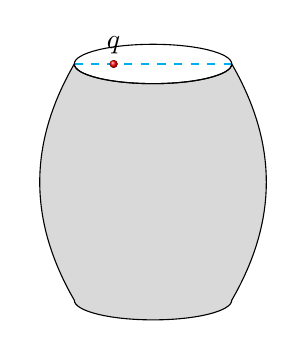
\begin{tikzpicture}[]
    \draw[fill=gray!30] (-1, 3) to[bend right] (-1, 0) arc(180:360:1 and 0.25) to[bend right] (+1, 3) arc(0:-180:1 and 0.25);
    \draw[dashed, cyan] (-1, 3) -- (+1, 3);
%    \draw (+1, 3) to[bend left] (+1, 0);
%    \draw (0, 0) circle (1 and 0.25);
    \draw (0, 3) circle (1 and 0.25);
     \fill [ball color=red] (-0.5, 3) circle (0.05) node[above] {$q$};
\end{tikzpicture}
\caption{До задачі~\ref{prb:potter}}
\label{pic:potter}
\end{minipage}
%---------------------------------------------------------
\begin{minipage}[t]{0.45\linewidth}\centering
    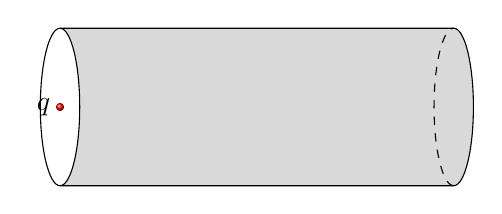
\begin{tikzpicture}
        \def\r{2}
        \draw [fill=gray!30] (0, {\r/2}) -- ++(5, 0) arc (90:-90:0.25 and {\r/2}) -- ++(-5, 0) arc (-90:+90:0.25 and {\r/2}) -- cycle;
        \draw (0, -{\r/2}) arc(270:90:0.25 and {\r/2});
        \draw[dashed] (5, -{\r/2}) arc(270:90:0.25 and {\r/2});
        \fill [ball color=red] (0, 0) circle (0.05) node[left] {$q$};
    \end{tikzpicture}
\caption{До задачі~\ref{prb:tube}}
\label{pic:tube}
\end{minipage}
%---------------------------------------------------------
\end{figure}
%=========================================================


%=========================================================
\begin{problem}\label{prb:flux_rotated_hemisphere}
nЗнайти потік індукції однорідного магнітного поля $\Bfield$ поверхню нахиленої напівкулі (рис.~\ref{pic:flux_rotated_hemisphere}). Вектор $\Bfield$
спрямований  вертикально; площина основи нахилена на кут $\alpha$ до горизонтальної площини.
\end{problem}

%---------------------------------------------------------
\begin{figure}[h!]\centering
    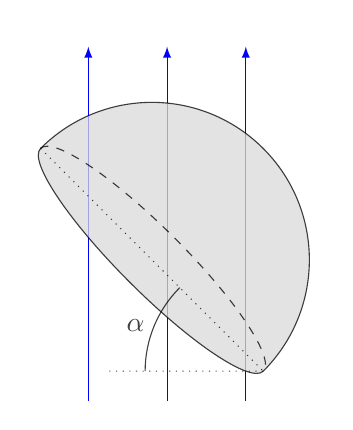
\begin{tikzpicture}[>=latex]
        \foreach[count=\c] \x in {0.9,...,3.6}{
            \draw[->, blue] (\x, -2.5) -- ++(0, 4.5)
            \ifnum\c=2
            node[above] {$\Bfield$}
            \fi
            ;
        }
        \begin{scope}[
            rotate around={-45:(1,0)},
            opacity=0.75]
            \draw[fill=gray!30] (0,0) arc (180:0:2) arc(0:-180:2 and {2*0.2});
        \draw[dashed] (0,0) arc (180:0:2 and {2*0.2});
        \draw[dotted] (0,0) -- (4,0);
        \draw[dotted] (4,0) -- ++(45:-2);
        \draw (4,0)  ++(-1.5,0) arc(180:{180+45}:1.5) node[pos=0.5, anchor=east] {$\alpha$};
        \end{scope}

    \end{tikzpicture}
\caption{}
\label{pic:flux_rotated_hemisphere}
\end{figure}
%---------------------------------------------------------

\end{document}
